\documentclass{article}

\usepackage[utf8]{inputenc}
\usepackage{graphicx}
\usepackage{caption}
\usepackage{subcaption}

\begin{document}

\begin{figure}
\centering
\begin{subfigure}[b]{1.2\textwidth}
\centering
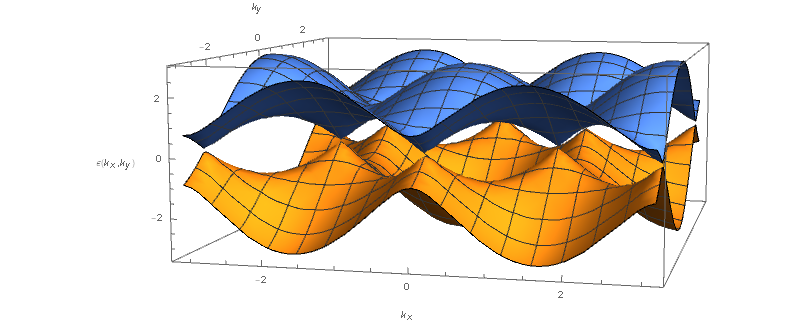
\includegraphics[width=\textwidth]{graphene_005.png}
\caption{$t'=0.05$}
\end{subfigure}	 
\begin{subfigure}[b]{1.2\textwidth}
\centering
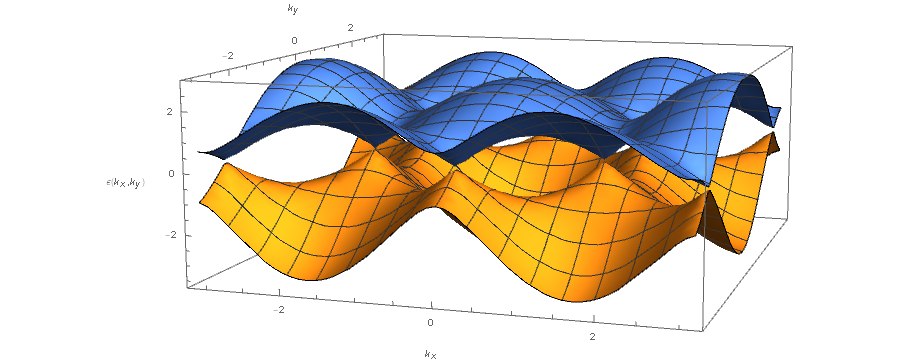
\includegraphics[width=\textwidth]{graphene_01.png}
\caption{$t'=0.05$}
\end{subfigure}	
\begin{subfigure}[b]{0.9\textwidth}
\centering
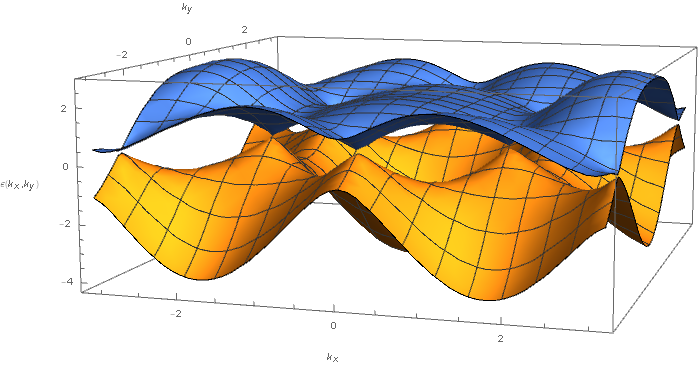
\includegraphics[width=\textwidth]{graphene_02.png}
\caption{$t'=0.05$}
\end{subfigure}	  
\end{figure}

\end{document}